\section{Error Analysis}
	We can find the RMS error in the reconstrcted matrix by using the following formula:

	$$\text{RMS Error} = \sqrt{\frac{1}{mn} \sum_{i=1}^{m} \sum_{j=1}^{n} (A_{ij}-A_{ij}^r)^2}$$
	
	Here, $A_{ij}$ is the original matrix and $A_{ij}^r$ is the reconstructed matrix.
	
	$$\text{\% RMS Error} = \frac{\text{RMS Error}}{256}100\%$$

	We divide the RMS error by 256 because the pixel values range from 0 to 255. So, the RMS error will be in the range of 0 to 255. We multiply the RMS error by 100 to get the percentage error.
		
	\begin{figure}[H]
		\centering
		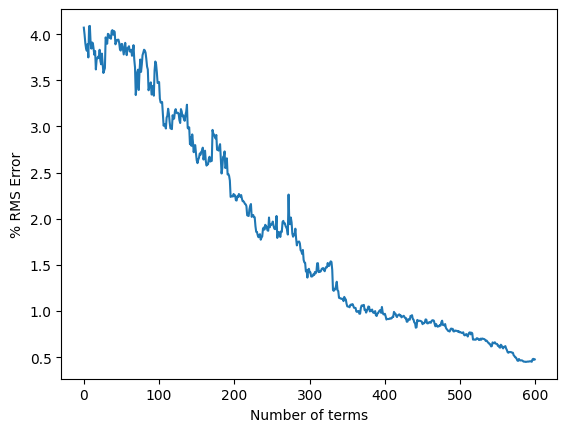
\includegraphics[width=0.4\textwidth]{../static/error_graph_grayscale.png}
		\caption{number of terms taken vs \% RMS error for the grayscale monkey image}
		\label{graph:grayscale_error}
	\end{figure}

	We have written a \href{https://github.com/PeithonKing/comp_phys_P346/blob/main/library/DIY.py#L37-L39}{\texttt{get\_rms\_error()}} function for calculating the percentage RMS error. It takes the original matrix and the reconstructed matrix as input and returns the percentage RMS error.

	We have created a graph for the percentage RMS error vs the number of singular values (terms) used. The graph for the grayscale monkey image is shown in \hyperref[graph:grayscale_error]{\textbf{Figure 5}} and for the color monkey image is shown in \hyperref[graph:color_error]{\textbf{Figure 6}}.
		
	\begin{figure}[H]
		\centering
		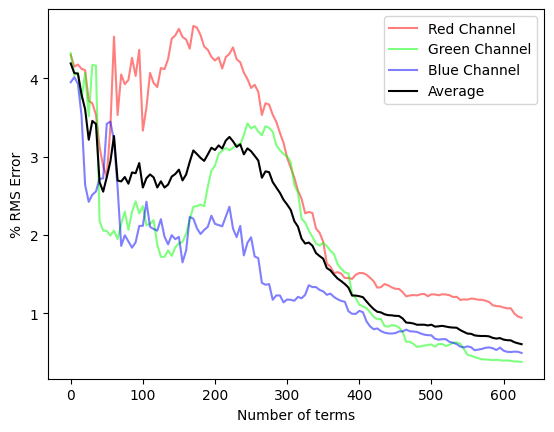
\includegraphics[width=0.4\textwidth]{../static/error_graph_colour.png}
		\caption{number of terms taken vs \% RMS error for the colour crab image}
		\label{graph:colour_error}
	\end{figure}


